\documentclass[11pt]{article}

\usepackage[margin=1in]{geometry}
\usepackage{booktabs}
\usepackage{graphicx}
\usepackage{enumitem}
\usepackage{hyperref}
\usepackage{xcolor}

\title{Island Escape: A Multi-Agent Survival Trading Game with LLM Negotiation}
\author{Yufeng He and Team}
\date{May 2026}

\setlist[itemize]{leftmargin=*, itemsep=0.25em}
\setlist[enumerate]{leftmargin=*, itemsep=0.25em}
\hypersetup{colorlinks=true, linkcolor=blue, urlcolor=blue}

\begin{document}

\maketitle

\begin{abstract}
Island Escape is a 2D survival trading game built around a simple question:
what happens when resource management is no longer only a numerical puzzle, but
also a social negotiation problem? The player is stranded on an island with four
AI-controlled characters. Every day, each character must gather food, decide
whether to sell resources to a merchant ship, negotiate with other islanders,
and survive the nightly resource drain. The first character to reach 100 coins
escapes.

Our main contribution is not just that we placed a language model inside a game.
The more important engineering decision was to keep the game state deterministic
and auditable while allowing the language model to influence high-level
intentions, dialogue, and bargaining behavior. The server remains the source of
truth. The LLM proposes actions and natural-language responses, but all resource
updates, phase transitions, trade execution, and win/loss checks are validated
by typed game logic. This gives us a game that feels social and emergent without
handing correctness to an unpredictable model.

During the final development stage, we extended the project with daily random
events, a day-scaled boss dungeon challenge, improved the negotiation interface,
clearer phase and resource feedback, and tighter validation across linting, type
checking, tests, and builds. The resulting prototype demonstrates an integrated
game loop: movement, resource labor, LLM-based negotiation, persistent game
state, real-time AI turn events, and an optional action-combat challenge that
creates a stronger final demo arc.
\end{abstract}

\section{Project Vision}

Island Escape began as a small survival economy, but the design target was
larger than a resource spreadsheet. We wanted a game where the interesting
decisions come from the interaction between three forces: scarcity, opportunity,
and social pressure. Scarcity comes from nightly fish and wheat consumption.
Opportunity comes from the merchant ship's fluctuating prices. Social pressure
comes from NPCs who have their own resources, incentives, and personalities.

The player is not simply optimizing a fixed formula. They need to decide when
to gather, when to sell, when to bargain, and when to take risks. The AI agents
turn that decision space into a more human-feeling negotiation game: Tom may be
cautious, Lily may cooperate, Sam may trade aggressively, and Jack may exploit
weakness. In practice, this makes the same mechanical state feel different
depending on who the player approaches and what they say.

My role in the project was to keep the design ambitious while making the
implementation robust enough for a live demo. I treated the LLM as an
unreliable collaborator rather than as a trusted database. That framing shaped
most of the architecture: typed shared schemas, server-side validation,
deterministic state transitions, guarded negotiation flows, and a UI that gives
the player immediate feedback when the model is thinking.

\section{Design Goals}

\subsection{A readable game loop}

The core loop needed to be understandable within a short presentation. We
therefore used a daily rhythm:

\begin{enumerate}
  \item the day starts, merchant prices refresh, and a daily event is rolled;
  \item the player must perform labor, either fishing or farming;
  \item the player spends up to two trade slots;
  \item AI agents take their turns;
  \item settlement consumes resources and checks elimination or escape.
\end{enumerate}

This structure gives the game a clean tactical cadence. The player always knows
what kind of decision they are making: survival first, trade second, then
consequences. Daily events add controlled variation without changing the phase
order.

\subsection{LLM agents with constrained authority}

The language model should make the characters feel alive, but it should not be
able to corrupt the game. In Island Escape, the model can decide what an NPC
wants to do and what it says, but it cannot directly mutate coins, fish, wheat,
friendship, or phase state. All of those updates pass through server-side game
engine functions.

This is an important engineering distinction. A naive LLM game often lets the
model narrate facts into existence. We avoided that. The model can propose a
trade. The server validates whether the resources exist. The model can accept a
proposal. The server decides which concrete proposal is executed. The model can
produce colorful text. The state machine decides whether the game advances.

\subsection{Presentation-first polish}

The final stage focused on making the demo reliable. In a classroom
presentation, a clever system is less convincing if the audience cannot see what
is happening. We therefore prioritized visible phase guidance, immediate
optimistic chat feedback while waiting for an LLM response, thinking states for
NPC dialogue, resource-change feedback, a boss dungeon for a more dramatic demo
moment, and validation commands that can be rerun before submission.

\section{Gameplay System}

\subsection{Resources and win condition}

Each character has fish, wheat, coins, trade slots, and status flags. Fish and
wheat are survival resources. Coins are the escape resource. The win condition
is deliberately simple: reach 100 coins and escape. The difficulty comes from
the fact that coins are not gathered directly. They must be obtained through
selling resources or by taking the risk of the dungeon reward.

\begin{table}[h]
\centering
\begin{tabular}{lll}
\toprule
Resource & Role & Main source \\
\midrule
Fish & Immediate survival resource & Fishing labor \\
Wheat & Delayed survival resource & Farming and harvest queue \\
Coins & Win-condition resource & Merchant sale, dungeon reward \\
Trade slots & Daily action budget & Reset each day \\
\bottomrule
\end{tabular}
\caption{Core resources in Island Escape.}
\end{table}

Fishing gives immediate fish. Farming creates a delayed wheat harvest. This
small asymmetry creates a useful tradeoff: the player can stabilize today or
invest in a later day. Because every character consumes resources at settlement,
running out of either fish or wheat eliminates them.

\subsection{Trade and negotiation}

Trading has two forms. The merchant ship is deterministic: the player sells fish
or wheat at the current day's prices. NPC negotiation is social: the player sends
a message and optionally attaches a structured proposal. The NPC responds
through the LLM, possibly with an offer, counter-offer, acceptance, or rejection.

The key design choice is that natural language and structured trade proposals
coexist. The text makes the interaction expressive. The structured proposal
makes it executable. If a player says, "I can give you fish," that may be
flavorful, but the server still needs exact amounts before resources can move.
This keeps the negotiation interface flexible without sacrificing correctness.

\subsection{Daily constraints}

Several constraints prevent trivial or broken play:

\begin{itemize}
  \item the player must labor before trading;
  \item trade actions only run during the trade phase;
  \item each day has a limited number of trade slots;
  \item a player cannot repeatedly trade with the same NPC in the same day;
  \item an active negotiation must be completed or closed before another starts;
  \item dungeon entry consumes a trade slot and is limited to once per day.
\end{itemize}

These checks are implemented server-side, not just in UI buttons. That matters
because the frontend can be bypassed, refreshed, or delayed by LLM calls. The
server is the authority.

\subsection{Daily random events}

The final gameplay pass adds a daily event system to make repeated days less
predictable. The event is stored in shared game state as
\texttt{dailyEvent}, rolled at dawn, written into the day-start log, and shown
in the HUD as a compact badge. The first two days are always calm so new players
can learn the loop before modifiers appear. Later days are still often calm, but
roughly one third introduce a rule change. The most punishing event, drought, is
suppressed until day 4 so early runs are not decided before players have wheat
buffers.

\begin{table}[h]
\centering
\begin{tabular}{lll}
\toprule
Event & Gameplay effect & Design role \\
\midrule
Calm day & Standard rules & Baseline economy \\
Storm & Fishing yields 2 fish instead of 3 & Pushes scarcity and trade \\
Festival & Peer-trade friendship gain is doubled & Rewards social play \\
Lucky Catch & Alive characters gain 2 fish at dawn & Recovery and tempo boost \\
Drought & Night upkeep costs 2 wheat & Punishes weak farming plans \\
\bottomrule
\end{tabular}
\caption{Daily event variants added to the core economy.}
\end{table}

These events are implemented inside deterministic game-engine functions rather
than by the LLM. For example, storm changes the result of fishing labor,
festival changes the friendship bonus after a peer trade, lucky catch grants
fish during day start, and drought changes the settlement cost. This keeps event
play visible and varied while preserving the same server-authoritative rule
model as the rest of the economy.

\section{AI Agent Design}

\subsection{Agent responsibilities}

The AI layer has two different jobs. First, AI agents take turns during the
simulation: they choose labor and trade actions. Second, NPCs respond during
negotiations with the player or with other AI agents. These are related but not
identical tasks.

For turn decisions, the model receives a state summary and produces a structured
decision: labor plus up to two trade choices. For negotiation, the model receives
the character context, the partner, current resources, personality, and dialogue
history. It then returns a short response and, when appropriate, a concrete
offer/request pair.

\subsection{Prompting philosophy}

The prompts were written to make the model behave like a game character rather
than a generic assistant. The system message asks for role-consistent behavior,
but the server still checks the result. This gives each NPC a different
behavioral tendency:

\begin{itemize}
  \item Tom is cautious and resource-protective.
  \item Sam is a fast, aggressive trader.
  \item Lily is cooperative and alliance-oriented.
  \item Jack is opportunistic and persuasive.
\end{itemize}

The important part is that these personalities affect negotiation style without
overriding the economy. If Jack wants to exploit the player, he still has to
make an executable trade.

\subsection{Model and provider boundary}

The project uses an OpenAI-compatible client. The current development
configuration is designed for DeepSeek through OpenRouter, using a model name
such as \texttt{deepseek/deepseek-chat}. This is intentionally abstracted behind
environment variables: \texttt{OPENAI\_API\_KEY},
\texttt{OPENAI\_BASE\_URL}, and \texttt{OPENAI\_MODEL}.

No real key belongs in the repository, report, slides, or screenshots. This is
both a security practice and a reproducibility practice: the code should explain
what variables are needed, but not leak a working credential.

\subsection{Handling LLM latency}

One final-demo issue we identified was that a player could send an NPC message
and not immediately see feedback. Because the LLM call may take a few seconds,
that makes the UI feel frozen even when the request is working. The frontend now
uses optimistic chat display and a pending/thinking state. The player's message
appears immediately, then the authoritative server response replaces the local
message list when it returns.

This is a small interaction detail, but it matters. Without it, the audience may
interpret model latency as a broken game. With it, latency becomes visible as
part of the AI interaction.

\section{Software Architecture}

\subsection{Monorepo layout}

The project is organized as a TypeScript monorepo:

\begin{itemize}
  \item \texttt{apps/web}: Vue 3 frontend, PixiJS canvas, 3D preview, UI state.
  \item \texttt{apps/server}: Fastify backend, game routes, LLM agent runtime,
  SQLite persistence.
  \item \texttt{packages/shared}: Zod schemas and shared TypeScript types.
\end{itemize}

This layout prevents the frontend and backend from drifting apart. Player
actions, game state, daily events, SSE events, and dungeon results are all
described in shared schemas. The server validates incoming actions against those
schemas, while the frontend receives inferred TypeScript types.

\subsection{Server as source of truth}

The backend owns the game state. The frontend sends actions to
\texttt{/api/games/:id/action}; the backend validates the action, updates the
state, persists it, and returns the new state. During AI turns, the backend also
broadcasts SSE events so the frontend can show progress without polling.

This design is deliberately conservative. In a game involving asynchronous LLM
calls, local UI state can easily become stale. By keeping the server
authoritative, we avoid confusing cases where the UI thinks a trade happened but
the resource ledger disagrees.

\subsection{State machine discipline}

Most game mechanics are implemented as explicit phase transitions:

\begin{itemize}
  \item \texttt{player\_labor}: only fishing or farming is valid.
  \item \texttt{player\_trade}: merchant trade, NPC negotiation, dungeon entry,
  or ending the turn is valid.
  \item \texttt{ai\_turns}: AI agents take labor/trade actions.
  \item \texttt{settlement}: resources are consumed and victory/elimination is
  checked.
\end{itemize}

This prevents ambiguous behavior. For example, an NPC negotiation should not
start during settlement. Dungeon results should not apply outside the dungeon
flow. The phase model makes these cases straightforward to reject.

\subsection{Persistence and real-time events}

Game sessions are kept in memory for active play and persisted to SQLite through
Drizzle. The frontend opens an SSE stream for each game. Events include state
updates carrying the daily event state, AI thinking, AI decisions, negotiation
lines, trade results, settlement events, eliminations, escapes, and dungeon
events.

This event model makes the game easier to present. The audience can see that AI
agents are not silent background calculations; they are taking turns, making
trades, and affecting the state.

\section{Boss Dungeon Extension}

The boss dungeon was added as a final-stage gameplay extension. The original
survival/trading loop is strategic but slow. For a short demo, we wanted one
high-energy moment that still connects to the economy. The dungeon does that.

Mechanically, the dungeon is an optional risk/reward action during the trade
phase:

\begin{itemize}
  \item entering costs one trade slot;
  \item only one run is allowed per day;
  \item winning grants a day-scaled coin reward;
  \item losing removes some fish and wheat;
  \item the player returns to the island flow afterward.
\end{itemize}

Inside the dungeon, the player fights a boss using movement, bullets, flash
movement, an ultimate skill, XP orbs, and upgrade cards. This gives the game a
second mode without replacing the main economy. The boss fight is not a separate
game pasted on top; it is another way to make an economic decision under risk.

The later boss update connects combat difficulty to the island day. When the
frontend enters dungeon mode, it passes the current day into
\texttt{DungeonArena}. The arena stores that value as a day level and passes it
to \texttt{Boss.setDifficulty}. Boss maximum HP increases by 50 per day, bullet
and charge damage increase by one per day with caps, attack cooldowns shrink
toward a lower bound, and minion spawn pacing, minion caps, and minion health
also scale upward. Clearing the dungeon also scales the reward by adding 4 coins
for each day after day 1, capped at 80 coins. This creates a real timing
tradeoff: entering early is safer but pays less, while delaying the dungeon can
accelerate escape but makes the fight more dangerous.

\section{Visual Rendering and Animation}

The final visual pass keeps the playable island and dungeon in PixiJS, while a
separate Three.js canvas renders the left-side interaction preview. This hybrid
approach improves presentation quality without moving tile logic, collision
checks, phase control, or server-authoritative game state into a 3D scene.

The preview reads the same interaction state as the action menu. It shows a
default island when no object is nearby, then swaps to procedural low-poly
models for fishing, farmland, merchant trading, NPC dialogue, and dungeon entry.
Each model rotates and floats subtly. The Three.js renderer caps device pixel
ratio, resizes with \texttt{ResizeObserver}, pauses when the document is hidden,
and disposes old geometry and materials when the active model changes.

\begin{figure}[htbp]
\centering
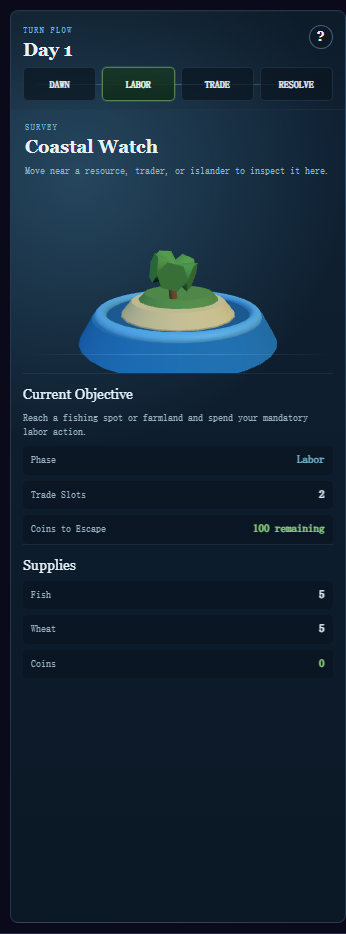
\includegraphics[height=0.34\textheight,keepaspectratio]{figures/panel-default-final.png}
\hspace{1em}
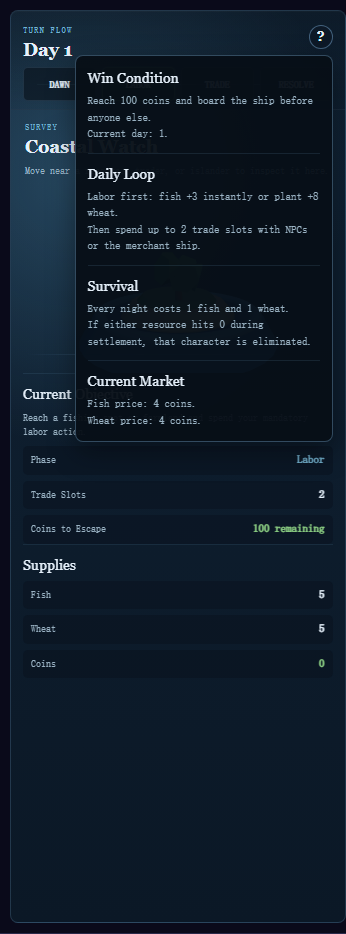
\includegraphics[height=0.34\textheight,keepaspectratio]{figures/panel-rules-topmost-final.png}
\caption{Left interaction panel in its default state and with the rules popover
open. The compact horizontal phase flow leaves more room for the 3D preview and
state-specific parameters.}
\end{figure}

The side panel now works as a contextual inspector rather than a decorative
preview. Fishing, farming, merchant, NPC, and dungeon states expose their
relevant parameters, such as yield, labor cost, harvest timing, market prices,
friendship, resources, and combat entry constraints. Longer phase and rules
descriptions are moved into hover popovers so the default layout stays compact.
The preview canvas has a 300-pixel minimum width, and popovers use a higher
stacking order so explanations remain visible above the model and parameter
grid.

Character labels were moved into a top PixiJS overlay layer rendered after the
tile, character, and effects layers. The labels use higher-resolution text,
stronger strokes, extra texture padding, and rounded pixel coordinates. This
keeps NPC names readable over terrain and animation effects.

\begin{figure}[htbp]
\centering
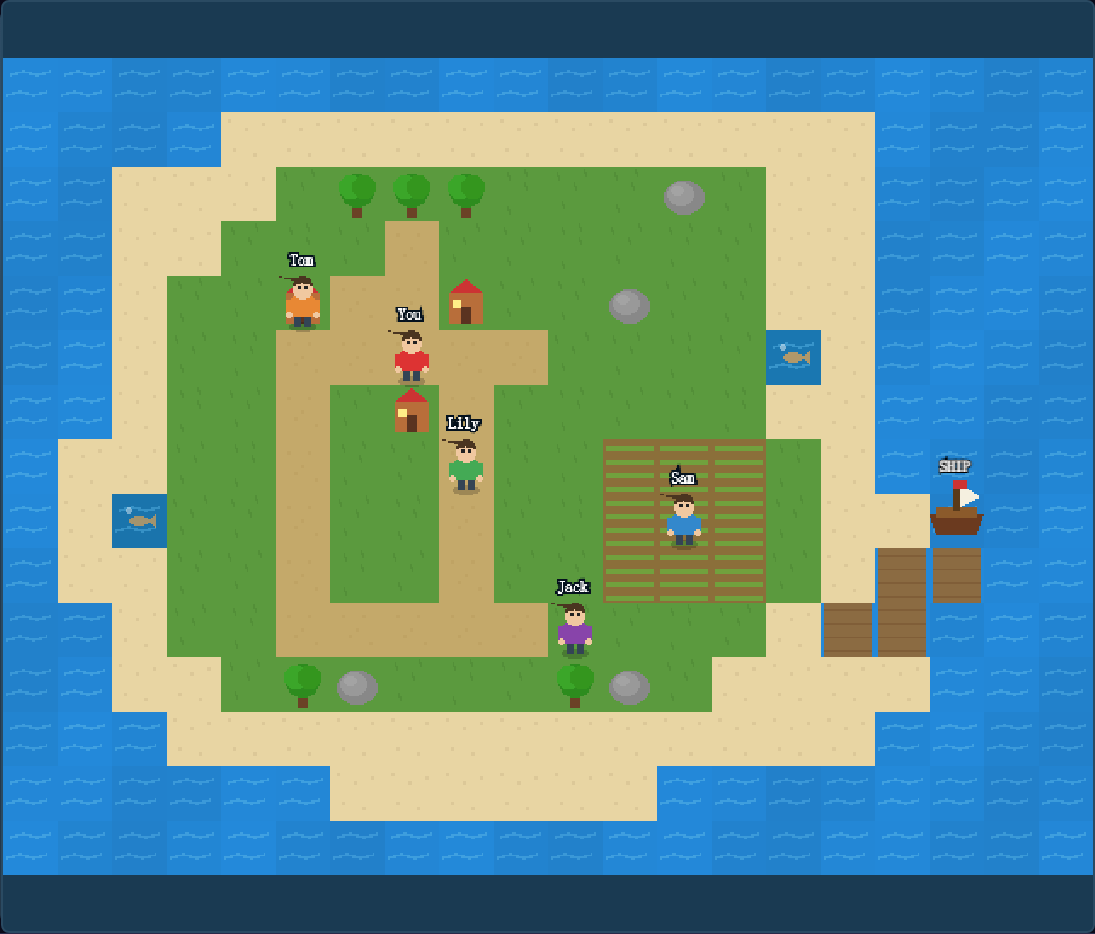
\includegraphics[width=0.9\linewidth,keepaspectratio]{figures/canvas-names-clarity.png}
\caption{Main canvas after the label-layer update. NPC names are rendered above
the world and remain sharp enough to identify characters during negotiation and
movement.}
\end{figure}

The dungeon reuses the same PixiJS application but switches from the island
container to \texttt{DungeonArena}. Its animation layer includes player combat,
boss states, pooled bullets, minions, XP orbs, hit sparks, damage numbers,
screen shake, hit-stop, flashes, vignette, and attack telegraphs. Browser
screenshots and frontend checks confirmed that the PixiJS/Three.js split made
the interface richer while preserving readable gameplay.

\section{Testing and Validation}

The project uses several validation layers:

\begin{itemize}
  \item schema tests in \texttt{packages/shared};
  \item backend API and game-flow tests in \texttt{apps/server};
  \item frontend unit tests for UI-derived state;
  \item TypeScript checks across the workspace;
  \item lint checks for frontend quality;
  \item production build validation through Vite and TypeScript.
\end{itemize}

\begin{table}[h]
\centering
\begin{tabular}{lll}
\toprule
Command & Purpose & Expected final status \\
\midrule
\texttt{pnpm lint} & static quality checks & Pass \\
\texttt{pnpm typecheck} & TypeScript correctness & Pass \\
\texttt{pnpm test} & unit/API/schema tests & Pass \\
\texttt{pnpm build} & production build & Pass with possible chunk-size warning \\
\bottomrule
\end{tabular}
\caption{Final validation checklist.}
\end{table}

One useful lesson from final integration was that passing unit tests alone was
not enough. After merging teammate work, the test suite passed, but typecheck
and build initially caught integration issues in shared state fields and helper
functions. Fixing those issues before submission improved the reliability of the
final demo and made the repository easier for teammates to continue.

\section{Team Contributions}

The final project was collaborative, but the work was not evenly distributed at
every stage. My contribution was strongest in system integration, AI architecture,
final stabilization, and preparing the materials needed for a credible
presentation.

\begin{itemize}
  \item \textbf{Yufeng He}: project coordination, report draft, presentation
  narrative, LLM/agent architecture direction, final integration, validation
  workflow, and demo-readiness checks.
  \item \textbf{Developer 1}: dialogue-related bug fixes and final PPT
  preparation based on the project proposal and new progress.
  \item \textbf{Erfei Yu}: daily event gameplay, boss dungeon feature work,
  day-scaled boss difficulty, flow polishing, and demo video recording/editing.
  \item \textbf{Zhiyuan}: visual rendering, animation, and 3D UI technical
  explanation for the report.
\end{itemize}

From an engineering perspective, the most important coordination decision was to
separate responsibilities late in the project. At that point, adding broad new
features would have been risky. We focused on a stable demo path: NPC dialogue,
resource/trade feedback, boss dungeon, report, PPT, and video.

\section{Limitations}

Island Escape is a prototype, and several limitations are still visible:

\begin{itemize}
  \item \textbf{LLM latency}: NPC responses can take several seconds depending
  on provider speed and network conditions.
  \item \textbf{Model variability}: different model outputs can change the tone
  and quality of negotiation, even under the same game state.
  \item \textbf{Balance}: daily events, dungeon scaling, merchant prices, and
  survival costs may need more playtesting.
  \item \textbf{Presentation risk}: a full game can be slow, so the final demo
  should combine a live short path with an edited video.
  \item \textbf{Visual asset depth}: the current 3D preview models are
  procedural, so authored models and textures could further improve fidelity.
\end{itemize}

\section{Future Work}

The most interesting future direction is to make the AI agents remember social
history more deeply. The current game has friendship and dialogue history inside
negotiations, but a richer version could track promises, betrayal, past prices,
and alliance formation across days.

Another direction is evaluation. Because LLM-driven games are partly subjective,
we should not only test code correctness. We should also measure whether players
understand the phase flow, whether negotiations feel fair, whether NPC
personalities are distinguishable, and whether the boss dungeon improves the
demo without distracting from the main AI-agent concept.

Finally, the dungeon and economy could be coupled more strongly. For example,
different NPC relationships could unlock cards, boss fights could change
merchant prices, or AI agents could react socially if the player repeatedly
chooses combat over cooperation.

\section{Conclusion}

Island Escape demonstrates how a small game can use LLM agents in a disciplined
way. The language model adds personality, negotiation, and emergence; the
state machine preserves correctness. That separation is the core engineering
lesson of the project.

The final prototype combines a readable survival economy, daily random events,
AI-driven NPC negotiation, real-time event updates, a polished interaction UI,
and a day-scaled boss dungeon that gives the presentation a stronger climax.
More importantly, the project shows a practical pattern for future AI games: let
the model create intent and expression, but let typed code own the rules.

\begin{thebibliography}{9}
\bibitem{park2023generative}
Joon Sung Park et al.
\textit{Generative Agents: Interactive Simulacra of Human Behavior}.
2023. \url{https://arxiv.org/abs/2304.03442}

\bibitem{aitown}
a16z-infra.
\textit{AI Town}. \url{https://github.com/a16z-infra/ai-town}

\bibitem{projectsid}
Project Sid. \textit{Multi-Agent AI Simulation Reference}. 2024.
\end{thebibliography}

\end{document}
